% -----------------------------------------------------------------
%		 				 Dynamic Models
% -----------------------------------------------------------------

\begin{tcolorbox}[colback=green!5!white,colframe=green!75!black,title=\textbf{Continuous Time Systems}]
	\textbf{Ordinary Differential Equations (ODE):}
	\begin{align*}
	\dot{ x } &= f( x(t), u(t), \epsilon(t), p)
	\end{align*}
	
	\textbf{Differential Algebraic Equations(DAE):}
	\begin{align*}
	\dot{ x } &= f( x(t), u(t), \epsilon(t), p)\\
	0 &= g(x, z).
	\end{align*}
	
	\textbf{LTI Sytem (ODE):}
	\begin{align*}
	\dot x &= Ax+Bu \quad y = Cx+Du \\
	G(s) &= C (sI-A)^{-1} B+D
	\end{align*}
\end{tcolorbox}


\begin{tcolorbox}[colback=green!5!white,colframe=green!75!black,title=\textbf{Numerical Integration Methods}]
	
	\textbf{Euler Integration Step}
	\begin{align*}
	\tilde{x}(t; x_{init}, u_{const}) &= x_{init} + t f(x_{init}, u_{const}), \quad t \in [0, \Delta t]\\
	\tilde{x}_{j+1} &= \tilde{x}_j + h f (\tilde{x}_j, u_{const}), \quad j = 0, ..., M - 1
	\end{align*}
	\begin{itemize}
		\item[-] Approximation becomes better by decreasing the step size h.
		\item[-] Concistency Error: $h^2$
		\item[-] Total Number of steps: $\Delta t / h$
		\item[-] Error in the final step of order $h \Delta t$
		\item[-] Linear in step size $\rightarrow$ order one
		\item[-] Taking more steps is more accurate but needs more computional time
	\end{itemize}
	
	\textbf{Runge-Kutta Method of Order Four}
	\begin{align*}
		k_1 &= f(\tilde{x}_j, u_{const})\\
		k_2 &= f(\tilde{x}_j, \frac{h}{2} k_1, u_{const})\\
		k_3 &= f(\tilde{x}_j, \frac{h}{2} k_2, u_{const})\\
		k_4 &= f(\tilde{x}_j, h k_3, u_{const})\\
		\tilde{x}_{j+1} &= \tilde{x}_j + \frac{h}{6} (k_1 + 2k_2 + 2k_3 + k_4)
	\end{align*}
	
	One Step of RK4 is thus as expensive as four steps of euler\\
	accurency of final approximation is of order $h^4 \Delta$ t\\
	$\rightarrow$ rk4 needs fewer functions to obtain the same accuracy level as euler
\end{tcolorbox}

\begin{tcolorbox}[colback=green!5!white,colframe=green!75!black,title=\textbf{Discrete Time Systems}]
	\begin{tabular}{ll}
		Det. Model as State Space  & Stoch. Model as State Space  \\
		Det. Model as Input-Output  & Stoch. Model as Input-Output 
	\end{tabular}
	
	\textbf{Deterministic Model}
	\todo[inline]{Erklaerung}
	
	\textbf{Finite Impulse Response (FIR): } 
	\begin{align*}
		y(k) &= b_0 u(k) + ... + b_{n_b} u(k-n_b) \\
		G(z) &= b_0 + b_1z^{-1} + ... + b_{n_b}z^{-n_b} \quad | \cdot \frac{z^{n_b}}{z^{n_b}} \\
		&= \frac{b_0 z^{n_b} + b_1 z^{ n_{b-1} } + ... + b_{n_b} }{z^{n_b}}
	\end{align*}
	
	\textbf{Auto Regressive Models with Exogenous Inputs (ARX): }
	\begin{align*}
		G(z) = \frac{b_0z^n + b_1z^{n-1} + \cdots + b_n}{a_0z^n + a_1z^{n-1} + \cdots + a_n}
	\end{align*}
	
	\textbf{LTI system as State-Space Model:}
	\begin{align*}
		x_{k+1} = A x_k + B u_k, \quad k = 0, 1,..., N - 1. 
	\end{align*}
	
	\textbf{LTI system as Input-Output Model:}
	\begin{flalign*}
		G(s) &= \frac{ b_0 + b_1s+...+b_ns^n }{ a_0+a_1s+...+a_{n-1}s^{n-1}+s^n } \quad | \cdot s = z^{-1} &\\
		G(z) &= \frac{ b_0 + b_1 z^{-1}+...+b_n z^{-n} }{a_0+a_1z^{-1}+...+a_n z^{-n}} &\\
		&= \frac{ b_0z^n+b_n z^{n-1}+...+b_n}{a_0 z^n+a_1 z^{n-1}+...+a_n} \quad \Rightarrow \text{Also called "polynomial model".} &
	\end{flalign*}	
	\textbf{Stochastic Model}
	\todo[inline]{Erklaerung}
	
	Assumptions:  noise is i.i.d.\\
	
	\textbf{State Space Model}
	\begin{align*}
	x(t+1) = f(x(k), u(k), \epsilon(k)) \\
	y(k) = g(x(k), u(k), \epsilon(k))
	\end{align*}
	
	\textbf{Input-Output Model}
	\begin{align*}
	y(k) &= h(u(k), ..., u(k-n), y(k-1), ..., y(k-n), \epsilon(k), ..., \epsilon(k-n))\\
	\text{for} \quad k &= n + 1, n + 2, ...
	\end{align*}
	
	
	\textbf{Measurement Noise (Output Error Model)}
	\begin{align*}
	y(k) = M(k; U, x_{init}, p) + \epsilon(k)
	\end{align*}
	\todo[inline]{Bild einfuegen}
	Non-Linear Model
	
	
	\textbf{Stochastic Disturbance (Equation Errors)}
	\begin{align*}
	y(k) &= h(p, u(k), ..., u(k-n), y(k-1), ..., y(k-n)) + \epsilon(k)\\
	for \quad k& = n + 1, n + 2, ...
	\end{align*}
	
	\textbf{Linear In the Parameters models (LIP):}
	\begin{align*}
	y(k) &= \sum_{ i = 1}^{d}\theta_i\phi_i(u(k)...,y(k-1),...)+\epsilon(k)\\
	y(k) &= \varphi(k)^T\theta + \epsilon(k) \quad \text{where} \, \varphi = (\phi_1(\cdot),... ,\phi_d(\cdot)) 
	\end{align*}
\end{tcolorbox}
\begin{tcolorbox}[colback=green!5!white,colframe=green!75!black,title=\textbf{Discrete Time Systems}]	
	\textbf{LIP-LTI Models with Equation Errors (ARX)}\\
	combining best of two worlds (LTI and LIP)
	\begin{align*}
	a_0y(k) + ...+a_{n_{a}}y(k-n_a) = b_0u(k) + ... + b_{n_{b}}u(k-n_b) + \epsilon(k)
	\end{align*}
	
	\textbf{Auto-regressive moving average with eXogeneous input (ARMAX):}
	\begin{align*}
	a_0y(k) + ... + a_{n_a}y(k-n_a)\\
	=\\
	b_0u(k) + ... + b_{n_b} u(k - n_b) + \epsilon(k) + c_1 \epsilon(k-1) + ... + c_{n_x} \epsilon(k-n_c)
	\end{align*}
	
	\textbf{Auto-regressive moving average without inputs (ARMA):}
	\begin{align*}
	a_0y(k) + ... + a_{n_a}y(k-n_a)\\
	=\\
	\epsilon(k) + c_1 \epsilon(k-1) + ... + c_{n_x} \epsilon(k-n_c)
	\end{align*}
	Where $c_i$ represent the noise coefficient
	Have to use non-linear leas squares with the unknown noise terms$ \epsilon(k-i)$
	
	\textbf{Difference Deterministic and Stochastic Models}
	\begin{align*}
	- &stochastic noise \epsilon(k)\\
	- &unknown but constant parameter p\\
	- &measured output y(k) depend on both, \epsilon(k) and p
	\end{align*}
\end{tcolorbox}

\begin{tcolorbox}[colback=purple!5!white,colframe=purple!75!black,title=\textbf{Pure Output Error (OE) Minimization}]
	Assume: i.i.d. gaussian noise only affecting output\\
	using non-linear least squares
	\begin{align*}
	\theta_{ML} =\underset{\theta}{\text{min}} \sum_{k=1}^{N} (y(k)-M(k;U, x_{init} p))^2
	\end{align*}
	
	\textbf{Output Error Minimization for FIR Models:}
	lead to convex problems, therefore global minimum can be found
	\begin{align*}
	y(k) &= (u(k), u(k-1), ..., u(k-n_{n_b})) \cdot \theta +\varepsilon(k) &\\
	&= \underset {\theta}{ \text{min} } \sum_{k=n_{b}+1}^{N} (y(k)-\underbrace{(u(k), u(k-1),... , u(k-n_{n_b}))}_{\text{Deterministic part can be expressed as}\, M(k; U, x_{init}, p)} \cdot \theta)^2 &
	\end{align*}
	
	They often need a very high dimension $n_b$ to obtain a reasonable fit. As a consequence ARX models are usually used instead.
	
	\textbf{Equation Error Minimization:}
	Assume: i.i.d. $\epsilon(k)$ noise enters the input-output equation as additive disturbance
	
	\begin{align*}
	y(k) &= h(p, u(k), ..., u(k-n), y(k-1), ..., y(k-n)) + \epsilon(k)\\
	\text{for} \quad k &= n + 1, n + 2
	\end{align*}
	
	if the i.i.d noise is gaussian, a maximum likelihood formulation to estimate the unknown parameter vector $\theta = p$ is given:
	
	\begin{align*}
	\theta_{ML} = \underset {\theta}{ \text{min} } \sum_{k = n + 1}^{N}{(y(k) - h(p, u(k), ..., y(k-1), ...)) )^2}
	\end{align*}
	u and k are known input and output measurements, and the algorithm minimises the so called \textbf{equation errors} or \textbf{prediction errors}.
	
	This problem is also known as \textbf{Prediction error minimisation(PEM)}
	Such a problem is convex if $p$ enters linearly in $f$, i.e. if the model is \textbf{linear-in-the-parameters (LIP)}
	
	
	
	\textbf{PEM of LIP Models}
	
	\begin{align*}
	y(k) &= \varphi(k)^T\theta + \epsilon(k)\\
	\quad \text{where} \, \varphi &= (\phi_1(\cdot),... ,\phi_d(\cdot))^T \text{are the regressor variables}
	\end{align*}
	
	considering this last expression, the prediction error minimisation(PEM) problem can be formulated as:
	
	\begin{align*}
	\underset{\theta}{\text{min}} \underbrace{\sum_{k=1}^{N} (y(k)-\varphi(k)^\text{T} \theta)^2}_{= \parallel y_N - \Phi_N \theta \parallel_2^2}
	\end{align*}
	Which can be solved using LLS $\theta^* = \Phi^+_N y_N$
	
	\textbf{Special Case: PEM of LIP-LTI Models with Equation Errors(ARX)}
	General ARX model equation
	\begin{align*}
	a_0y(k)+...+a_{n_{a}}y(k-n_a) = b_0u(k)+...+b_{n_{b}}u(k-n_b)+\epsilon(k)
	\end{align*}
	
	In order to have a determined estimation problem, $a_0$ has to be fixed, otherwise the number of optimal solutions would be infinitive. Therefore we sually fix $a_0 = 1$ and use $\theta = (a_1, ..., a_{n_a}, b_0, ..., b_{n_b})^\text{T}$ as the parameter estimation vector. The regressor vector is given by:
	\begin{align*}
	\varphi = (-y(k-1), ..., -y(k-n_a), u(k), ..., u(k-n_b))^\text{T}
	\end{align*}
	leading to the optimal solution provided by LLS:
	\begin{align*}
	y(k) = \varphi(k)^\text{T} \theta + \epsilon(k)
	\end{align*}
	
\end{tcolorbox}
\begin{tcolorbox}[colback=purple!5!white,colframe=purple!75!black,title=\textbf{Pure Output Error (OE) Minimization}]
	\textbf{Models with Input and Output Errors:}
	
	\begin{align*}
	y(k)=M(k;U + \varepsilon_{N}^{u}, x_{init}, p) + \epsilon^y(k)
	\end{align*}
	
	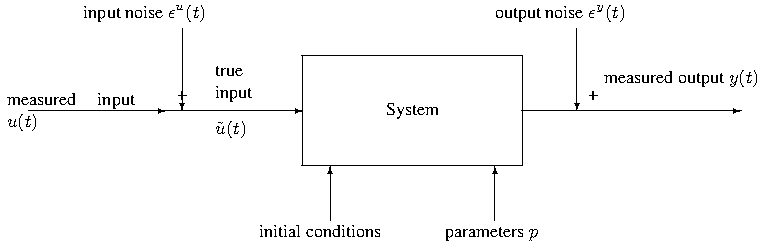
\includegraphics[width=\textwidth]{model.pdf}
	
	Assume: i.i.d. gaussian noise on both input and output with variance $\sigma_u^2$ for the input and $\sigma_y^2$ for the output
	
	\begin{align*}
	& \underset{\theta}{arg\,min} \sum_{k-1}^{N} \frac{1}{\sigma_{y}^{2}} (y(k)-M(k;U+ \epsilon_{N}^{u},x_{init},p))^2 + \frac{1}{\sigma_{u}^{2}} (\epsilon_u (k))^2 & \\
	& \underset{\theta}{arg\,min} \sum_{k-1}^{N} \frac{1}{\sigma_{y}^{2}} (y(k)-M(k;\tilde U, x_{init}, p))^2 + \frac{1}{\sigma_{u}^{2}} (u(k)-\tilde u(k) )^2 &
	\end{align*}
	
	
\end{tcolorbox}
